\section{Свёрточные нейронные сети}


Свёрточные нейронные сети (Convolutional Neural Network, CNN)- незаменимый инструмент для решения подавляющего большинства задач компьютерного зрения. 
На сегодняшний день существует множество различных архитектур, нацеленных на решение той или иной задачи. 
Очень часто свёрточные сети применяют как экстрактор признаков - сеть, которая предобучена извлекать признаки из изображения. К получившейся 
на выходе из такой сети матрице, называемой карте признаков(feature map), можно применять дополнительные преобразования для решения конкретной задачи. 

В рассмотренных нами подходах к решению задачи выявления заметных объектов на изображении свёрточные нейронные сети 
применяются и как самостоятельная модель, и в качестве экстрактора признаков. Однако, основные составные части свёрточной сети 
остаются практически неизменными. В этой главе будут описаны основные операции, характерные для архитектуры свёрточной нейронный сети,
а также рассмотрены архитектуры ResNet-50\cite{ResNet} и Efficient-Net b0 \cite{Efficientnet}, которые будут использованы в качестве 
экстракторов в экспериментах с моделью BBS-Net \cite{BBS}


\subsection{Основные операции}
Основные операции, или слои, в свёрточнах нейронных сетях - это идущие последовательно операции свёртки, активации и пулинга. Блоки из свёртки и операции
обычно повторяются несколько раз перед применением пулинга \cite{ResNet}. Рассмотрим эти операции подробнее.

\subsubsection{Операция свёртки}

\begin{figure}[h]
    \centering
    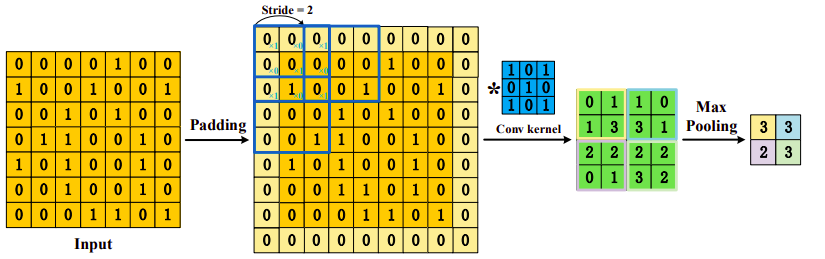
\includegraphics[width=0.7\textwidth]{conv_and_pool}
    \caption{Пример 2D операции свёртки и следующей за ней операции субдискретизации}
    \label{fig:conv}
\end{figure}


Свёрточный слой - основной строительный блок свёрточной нейронной сети. Каждый слой, реализующий операцию свёртки,
содержит несколько матриц с параметрами установленного размера, называемых ядрами.Каждое из ядер применяется ко входной карте 
активации и с некотором шагом проходит по всей карте: оно умножается на параметры входной карты, попавшей в окно, вдоль всех каналов.
Затем полученные значения складывается их друг с другом и записываются как один элемент в новую карту признаков в соответствующий канал. 
Такие ядра являются обучаемыми параметрами слоя и образуют новые каналы.
Пример применения свёрточного слоя изображён на \ref{fig:conv}.


Обычно рецептивное поле операции свёртки - то есть группа чисел в карте признаков, попадающая под действие свёртки -
соответствует форме и размеру ядра, например квадрату $3 \time 3$. Однако, существует более общий вид,
называемый расширенной свёрткой(dilated convolution)\cite{Dilated}. У таких свёрток рецептивное поле контролируется параметром скорости
расширения (dilation rate). Так, для стандартной свёртки он равен 1. Если параметр равен 2, то рецептивное поле увеличивается
до размера $7 \time 7$, как показано на изображении \ref{fig:dilated}

\begin{figure}[h]
    \centering
    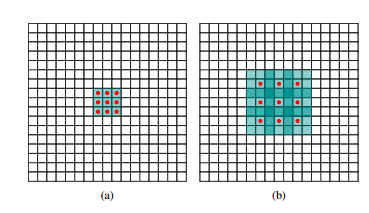
\includegraphics[width=0.7\textwidth]{dilated}
    \caption{Пример расшеренной свёртки.     (a) параметр dilation rate равен 1, что соответствует обычной свёртке. (b) параметр dilation rate равен 2}
    \label{fig:dilated}
\end{figure}


\subsubsection{Операция Субдискретизации}

Операция субдискретизации, или операция пулинга(Pooling), представляет собой операцию уменьшения размерности входящей карты признаков 
путём применения некоторой стратегии. Самой распространённой стратегией является стратегия максимально пулинга(Max Pooling),
при которой из группы соседних чисел, например внутри квадрата $2 \times 2$, выбирается максимальное и записывается в новую
карту признаков. Пример применения слоя пулинга изображён на \ref{fig:conv}.


Операция пулинга может быть записана следующим образом:

\begin{equation}
    f_{x,y}(S) = \max_{a,b=0}^{s}S_{sX+a, sY+b}
\end{equation}

где $S$ - карта активации, $s$ - размер окна.

\subsubsection{Функция активации ReLU}

\begin{figure}[h]
    \centering
    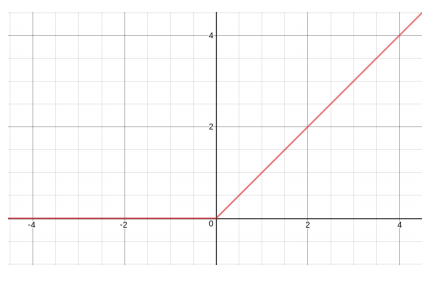
\includegraphics[width=0.7\textwidth]{relu}
    \caption{Функция ReLU}
    \label{fig:relu}
\end{figure}

Обычно, после применения свёртки, следующим шагом идёт применение функции активации для добавления нелинейности. Таким образом,
несколько последовательных свёрток, являясь линейными операциями, не будут эквивалентны одной свёртке, а будут описывать действительно 
разные признаки объекта. Одной из самых популярных функций активаций стала функция ReLU(Rectified Linear Unit) \cite{ReLU}, которая определяется
как. График функции ReLU изображён на \ref{fig:relu}.

\begin{equation}
    f(x) = max(0,x)
\end{equation}


\subsubsection{Пакетная нормализация}

Пакетная нормализация (Batch Normalization) - метод, позволяющий сделать 
нейронную сеть более устойчивой и производительной. Он был предложен в 
работе \cite{Batch-Norm}. Идея метода в предварительной нормализации
и центрировании карт признаков, подающихся на определённые слои сети.
Кроме того, слой также имеет обучаемые параметры масштабирования
и сдвига.

Пакетная нормализация может быть выражена следующим образом.
На вход слою пакетной нормализации BN поступает пакет объектов-признаков:
$B = (x_1 \dots x_m)$. На выходе каждому объекту $x_i, i \in \{1 \dots m\}$
ставится в соответствие значение $y_i$:
\begin{equation}
    y_i = BN_{\gamma, \beta}(x_i) = \gamma \hat{x_i} + \beta
\end{equation}

где $\gamma$ и $\beta$ - обучаемые параметры масштабирования и сдвига соответственно,
а 

\begin{equation}
    x_i = \frac{x_i - \mu_B}{\sqrt{\sigma_B^2 + \epsilon}} \text{ где} \\
\end{equation}

где $\mu_B$ - выборочной среднее по пакету: 

\begin{equation}
    \mu_B = \frac{1}{m}\sum_{i=1}^{m}x_i 
\end{equation}

а $\sigma_B^2$ - выборочная дисперсия:

\begin{equation}
    \sigma_B^2 = \frac{1}{m}(x_i - \mu_B)^2
\end{equation}


\subsection{Экстракторы признаков}

Для того, чтобы работать с изображением, его необходимо преобразовать
в некоторую матрицу, хранящую признаки. На основе этих 
признаков мы можем решать задачи классификации, распознавая что изображено на изображении,
детекции и сегментации, делая вывод о местоположении этого объекта,
а также огромное число других задач компьютерного зрения, в том числе и задачу SOD.

Именно для извлечения этих признаков и используются предобученные свёрточные сети, называемые экстракторами признаков. Они позволяют 
абстрагироваться от построения процесса извлечения признаков и сосредоточиться на решении конкретной задачи.
Более того, использование экстракторов существенно сокращает время тренировки и необходимые для неё мощности,
ведь веса экстрактора уже обучены и могут быть заморожены во время обучения, а обучать можно только специальные добавленные слои.


В данной работе мы будем использовать свёрточные сети ResNet-50\cite{ResNet} и EfficientNet-B0\cite{Efficientnet} 
в качестве бекбона для сети BBS-Net\cite{BBS}. Ниже рассмотрим основные особенности этих сетей.

\subsubsection{ResNet-50}

Архитектура ResNet была предложена в работе \cite{ResNet} и произвела настоящую революцию 
в изучении и проектировании свёрточных нейронных сетей. Главная отличительная особенность данной архитектуры -
блоки с остаточными связями (residual connection blocks) вида

\begin{equation}
    y = F(x, \{W_i\}) + x 
\end{equation}

где $x$ и $y$ - соответственно входной и выходной векторы. Функция $F(x, \{W_i\})$ отображает 
функцию, содержащую обучаемый параметр $W_i$. Например, на рисунке \ref{fig:resnet} функция $F$ 
представляет собой композицию функций умножения матриц и функции активации:
\begin{equation}
    F = W_2 \sigma(W_1x)
\end{equation}
где $\sigma$ - обозначает функцию активации ReLU\cite{ReLU}

\begin{figure}[h!]
    \centering
    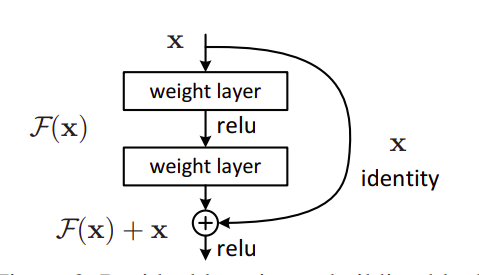
\includegraphics[width=0.7\textwidth]{resnet.png}
    \caption{Блок с остаточными связями (Residual Connection Block)}
    \label{fig:resnet}
\end{figure}

Подобное улучшение позволило обучать гораздо более глубокие свёрточные сети. 
В работе были представлены несколько модификаций сети ResNet, отличающихся глубиной.
В \cite{BBS} была использована сеть ResNet-50 в качестве экстрактора для сети BBS-Net. В нашей работе 
мы также проведём несколько экспериментов с этим экстрактором.

\subsubsection{Efficient-Net}

Архитектура EfficientNet была представлена в работе \cite{Efficientnet}. Авторы статьи предлагали метод 
балансирования различных гиперпараметров свёрточной нейронной сети, таких как разрешение, количество каналов  и число слоёв.
В работе \cite{Efficientnet} было представлено несколько моделей, основанных на различных архитектурах свёрточных сетей
и улучшенных предложенным методом.

В нашей работе мы будем использовать архитектуру EfficientNet-B0 как самую легковесную среди предложенных.
Она основана на архитектуре сети MobileNetV2 \cite{MobileNetV2}. На графике \ref{fig:effent} из работы \cite{Efficientnet}
изображена зависимость точности от размера различных свёрточных сетей. Видно, что обладая гораздо меньшим размером 
по сравнению с ResNet-50, EfficientNet-B0 обгоняет её в точности.

 \begin{figure}[h!]
    \centering
    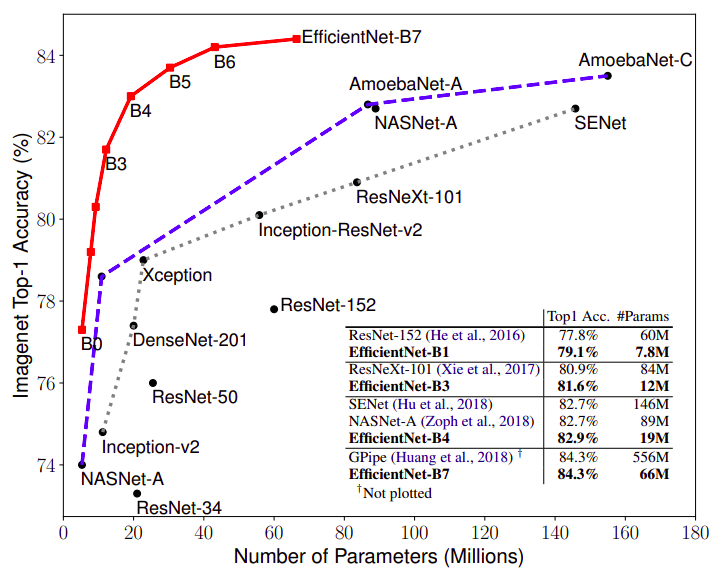
\includegraphics[width=0.7\textwidth]{effnet.png}
    \caption{График зависимости точности моделей от размера из работы \cite{Efficientnet}}
    \label{fig:effent}
\end{figure}

В нашей работе мы попробуем использовать более легкую по сравнению с ResNet-50 сеть EfficientNet-B0 в качестве экстрактора признаков для BBS-Net
и сравним точность полученной модели.
